\chapter{Din\'{a}mica y Cinem\'{a}tica}\label{sec:Modelado}

\section{Descripci\'{o}n del Sistema}\label{sec:desdelsist}



Para desarrollar el modelo matem\'{a}tico del gimbal definiremos cuatro sistemas de coordenadas. Primeramente necesitamos un marco inercial,
para ello consideraremos la tierra como plana y estacionaria en un espacio
inercial, por lo que cualquier sistema coordenado o marco de referencia fijo en la misma es por ende un sistema inercial en el que las
leyes de newton son validas. Lo anterior es necesario para poder desarrollar
las ecuaciones de movimiento del gimbal de tal manera que denotaremos al
marco de referencia fijo en la tierra como el marco $\left( E\right) $
definido por los vectores unitarios $\left\{ \hat{I}_{E},\hat{J}_{E},%
\hat{K}_{E}\right\} ,$ donde su origen esta ubicado arbitrariamente en
la superficie de la tierra para ajustarse a las circunstancias del problema,
el eje $O_{E}\hat{K}_{E}$ apunta verticalmente hacia abajo y el eje $%
O_{E}\hat{I}_{E}$, el cual es horizontal se elije en cualquier direcci\'{o}n
conveniente, por ejemplo el norte o sobre un camino, o en alguna direccion
de referencia de vuelo.

Denotaremos el marco de referencia del cuerpo como $\left( B\right) $,
definido por los vectores unitarios $\left\{ \hat{\imath}_{B},\hat{\jmath}%
_{B},\hat{k}_{B}\right\} $ este marco esta fijo al fuselaje del aeronave
y consideraremos que se encuentra cerca de su centro de gravedad ver figura \ref{fig:RefFra}.

El marco que se encuentra fijo al eslab\'{o}n externo del gimbal lo
denotaremos como $\left( P\right) $, definido por el el conjunto de vectores
unitarios $\left\{ \hat{\imath}_{P},\hat{\jmath}_{P},\hat{k}_{P}\right\} 
$, este marco rota un \'{a}ngulo $ \eta $ alrededor del eje $\hat{k}_{B}$%
, a esta rotaci\'{o}n se le denomina \textit{"panning"}\ que se refiere a
una rotaci\'{o}n en el plano horizontal (azimut) de la c\'{a}mara (rotaci%
\'{o}n de gui\~{n}ada o \textit{"yaw"} en el aeronave).

Finalmente definimos el marco $\left( T\right) $ el cual es el marco de
referencia del eslab\'{o}n interno del gimbal y esta definido por los
vectores unitarios $\left\{ \hat{\imath}_{T},\hat{\jmath}_{T},\hat{k}%
_{T}\right\} $, este eslab\'{o}n rota un \'{a}ngulo $\varepsilon $ alrededor
del eje $\hat{\jmath}_{P}$ del eslab\'{o}n externo, esta rotaci\'{o}n es
denominada como elevaci\'{o}n o "tilting" que se refiere a una rotaci\'{o}n
de la camara en un plano vertical (rotaci\'{o}n de cabeceo o \textit{"pitch"}
en el aeronave).

\begin{figure}[thpb]
      \centering
      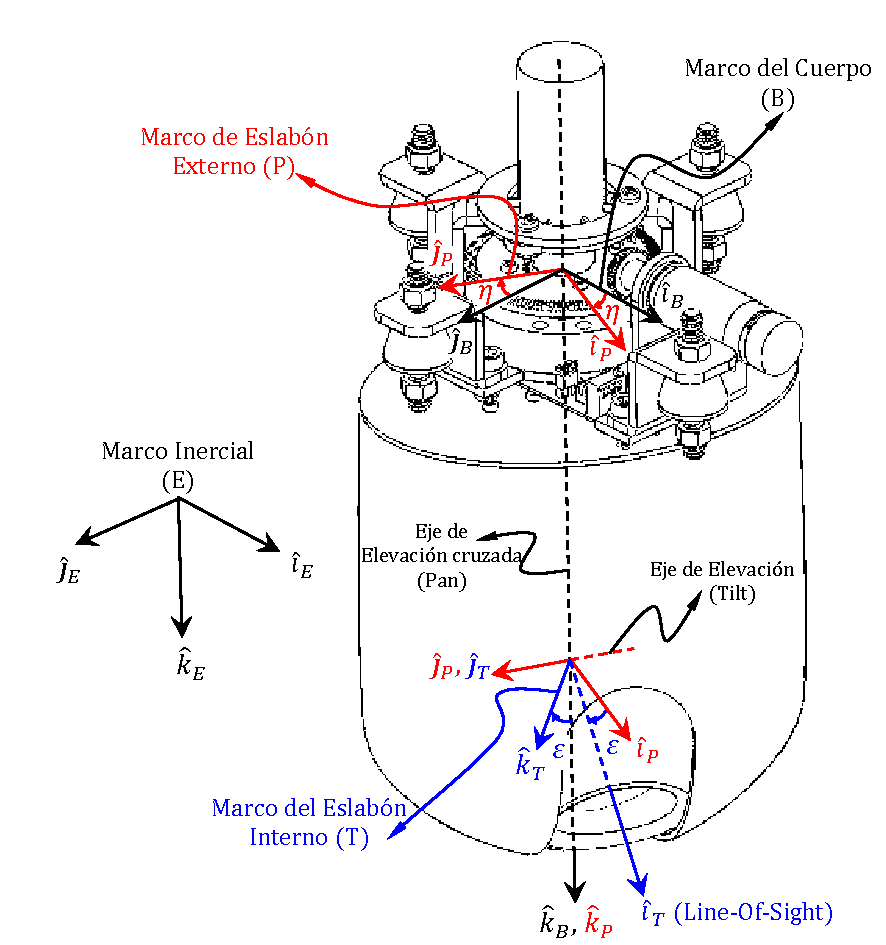
\includegraphics[scale=0.7]{img/Gimbal_Frames.pdf}
      \caption{Marcos de referencia del sistema gimbal}
      \label{fig:RefFra}
   \end{figure}

\section{Cin\'{e}matica}

Las velocidades \'{a}ngulares de los marcos $\left( P\right) $ y $\left(
T\right) $ son nuestras variables a controlar, el control de elevaci\'{o}n
se hace a traves del eslav\'{o}n interno, mientras que el control en el
plano horizontal (azimut) se hace a traves del eslab\'{o}n externo. Es
importante notar que la estabilizaci\'{o}n se requiere en el eje $\hat{\jmath%
}_{T}$ del eslab\'{o}n interno del gimbal denominado \textit{"elevaci\'{o}n
transversal"}; la estabilizaci\'{o}n se necesita en este eje puesto que es
en donde esta montada la c\'{a}mara, pero como antes se menciono la rotaci%
\'{o}n en azimut se controla con el eslab\'{o}n externo por lo que en
realidad la elevaci\'{o}n transversal es controlada indirectamente ya que el actuador esta montado en el eje $\hat{k}_{P}$ del eslab\'{o}n externo.

\subsection{Transformaciones b\'{a}sicas entre marcos de referencia}

Todos los marcos de referencia est\'{a}n relacionados por matrices de
transformaci\'{o}n, las cuales esta\'{a}n definidas como la suma de una matriz de traslaci\'{o}n
y una de rotaci\'{o}n. Considerando que nuestro inter\'{e}s se centra en velocidades \'{a} y aceleraciones \'{a}ngulares y \'{a}ngulos, y debido a que la
distancia que existe entre un marco y otro no afecta la forma en la que el
vector de velocidad de un marco se relaciona con otro, podemos despreciar esta distancia y considerar que el marco $%
\left( P\right) $ y $\left( T\right) $ tienen el mismo origen que $\left(
B\right) $ y de esta manera evitar utilizar la matriz de traslaci\'{o}n simplificando los c\'{a}lculos.

La matriz de rotaci\'{o}n que relaciona el marco de referencia $\left(
P\right) $ con respecto a $\left( B\right) $, la obtenemos calculando los
cosenos directores, de tal forma que:

\begin{equation*}
R_{B}^{P}=\left[ 
\begin{array}{lll}
\hat{\imath}_{P}\cdot \hat{\imath}_{B} & \hat{\jmath}_{P}\cdot \hat{\imath}%
_{B} & \hat{k}_{P}\cdot \hat{\imath}_{B} \\ 
\hat{\imath}_{P}\cdot \hat{\jmath}_{B} & \hat{\jmath}_{P}\cdot \hat{\jmath}%
_{B} & \hat{k}_{P}\cdot \hat{\jmath}_{B} \\ 
\hat{\imath}_{P}\cdot \hat{k}_{B} & \hat{\jmath}_{P}\cdot \hat{k}_{B}
& \hat{k}_{P}\cdot \hat{k}_{B}%
\end{array}%
\right]
\end{equation*}

\begin{equation*}
=\left[ 
\begin{array}{ccc}
\left\Vert \hat{\imath}_{P}\right\Vert \left\Vert \hat{\imath}%
_{B}\right\Vert \cos (\eta )\text{ \ \ \ \ \ \ \ } & \left\Vert \hat{\jmath}%
_{P}\right\Vert \left\Vert \hat{\imath}_{B}\right\Vert \cos (90+\eta ) & 
\left\Vert \hat{k}_{P}\right\Vert \left\Vert \hat{\imath}_{B}\right\Vert
\cos (90) \\ 
\left\Vert \hat{\imath}_{P}\right\Vert \left\Vert \hat{\jmath}%
_{B}\right\Vert \cos (90-\eta ) & \left\Vert \hat{\jmath}_{P}\right\Vert
\left\Vert \hat{\jmath}_{B}\right\Vert \cos (\eta )\text{ \ \ \ \ \ \ } & 
\left\Vert \hat{k}_{P}\right\Vert \left\Vert \hat{\jmath}_{B}\right\Vert
\cos (90) \\ 
\left\Vert \hat{\imath}_{P}\right\Vert \left\Vert \hat{k}_{B}\right\Vert
\cos (90)\text{ \ \ \ \ } & \left\Vert \hat{\jmath}_{P}\right\Vert
\left\Vert \hat{k}_{B}\right\Vert \cos (90)\text{ \ \ \ } & \left\Vert 
\hat{k}_{P}\right\Vert \left\Vert \hat{k}_{B}\right\Vert \cos (0)%
\text{ }%
\end{array}%
\right]
\end{equation*}

Usando la identidad trigonom\'{e}trica $\cos (a\pm b)=\cos (a)\cos (b)\mp \sin
(a)\sin (b)$:

\begin{equation*}
R_{B}^{P}=\left[ 
\begin{array}{ccc}
\cos (\eta )\text{ \ \ \ \ \ \ \ } & \cos (90)\cos (\eta )-\sin (90)\sin
(\eta ) & 0 \\ 
\cos (90)\cos (\eta )+\sin (90)\sin (\eta ) & \cos (\eta )\text{ \ \ \ \ \ \ 
} & 0 \\ 
0\text{\ \ \ } & 0\text{\ \ } & 1\text{ }%
\end{array}%
\right]
\end{equation*}

obtenemos finalmente:

\begin{equation}
R_{B}^{P}=\left[ 
\begin{array}{ccc}
c\eta & -s\eta & 0 \\ 
s\eta & c\eta & 0 \\ 
0\text{\ \ \ } & 0\text{\ \ } & 1\text{ }%
\end{array}%
\right] ;\text{ \ \ \ \ }c\eta =\cos (\eta );\text{ }s\eta =\sin (\eta )%
\text{\ \ }
\label{eq:R_P_B}
\end{equation}

Empleando las propiedades b\'{a}sicas de la matriz de rotaci\'{o}n,
obtenemos la relaci\'{o}n del marco de referencia $\left( B\right) $ con
respecto a $\left( P\right) $:

\begin{equation}
R_{P}^{B}=\left( R_{B}^{P}\right) ^{-1}=\left( R_{B}^{P}\right) ^{T}=\left[ 
\begin{array}{ccc}
c\eta & s\eta & 0 \\ 
-s\eta & c\eta & 0 \\ 
0\text{\ \ \ } & 0\text{\ \ } & 1\text{ }%
\end{array}%
\right]
\label{eq:R_B_P}
\end{equation}

De la misma manera obtenemos a continuaci\'{o}n la relaci\'{o}n del marco de
referencia $\left( P\right) $ con respecto a $\left( T\right) $:

\begin{equation*}
R_{T}^{P}=\left[ 
\begin{array}{ccc}
\hat{\imath}_{T}\cdot \hat{\imath}_{P} & \hat{\jmath}_{T}\cdot \hat{\imath}%
_{P} & \hat{k}_{T}\cdot \hat{\imath}_{P} \\ 
\hat{\imath}_{T}\cdot \hat{\jmath}_{P} & \hat{\jmath}_{T}\cdot \hat{\jmath}%
_{P} & \hat{k}_{T}\cdot \hat{\jmath}_{P} \\ 
\hat{\imath}_{T}\cdot \hat{k}_{P} & \hat{\jmath}_{T}\cdot \hat{k}_{P}
& \hat{k}_{T}\cdot \hat{k}_{P}%
\end{array}%
\right]
\end{equation*}

\begin{equation*}
\left[ 
\begin{array}{ccc}
\left\Vert \hat{\imath}_{T}\right\Vert \left\Vert \hat{\imath}%
_{P}\right\Vert \cos (\varepsilon )\text{ \ \ \ \ \ \ \ \ \ \ \ } & 
\left\Vert \hat{\jmath}_{T}\right\Vert \left\Vert \hat{\imath}%
_{P}\right\Vert \cos (90)\text{ \ \ } & \left\Vert \hat{k}%
_{T}\right\Vert \left\Vert \hat{\imath}_{P}\right\Vert \cos (90+\varepsilon )
\\ 
\left\Vert \hat{\imath}_{T}\right\Vert \left\Vert \hat{\jmath}%
_{P}\right\Vert \cos (90)\text{ \ \ \ \ \ \ \ \ } & \left\Vert \hat{\jmath}%
_{T}\right\Vert \left\Vert \hat{\jmath}_{P}\right\Vert \cos (0)\text{ \ \ \ }
& \left\Vert \hat{k}_{T}\right\Vert \left\Vert \hat{\jmath}%
_{P}\right\Vert \cos (90)\text{ \ \ \ \ } \\ 
\left\Vert \hat{\imath}_{T}\right\Vert \left\Vert \hat{k}_{P}\right\Vert
\cos (90-\varepsilon ) & \left\Vert \hat{\jmath}_{T}\right\Vert \left\Vert 
\hat{k}_{P}\right\Vert \cos (90) & \left\Vert \hat{k}_{T}\right\Vert
\left\Vert \hat{k}_{P}\right\Vert \cos (\varepsilon )\text{ \ \ \ \ }%
\end{array}%
\right]
\end{equation*}

\begin{equation*}
=\left[ 
\begin{array}{ccc}
\cos (\varepsilon ) & 0 & \cos (90)\cos (\varepsilon )-\sin (90)\sin
(\varepsilon ) \\ 
0 & 1 & 0 \\ 
\cos (90)\cos (\varepsilon )+\sin (90)\sin (\varepsilon ) & 0 & \cos
(\varepsilon )%
\end{array}%
\right]
\end{equation*}

obtenemos finalmente:

\begin{equation}
R_{T}^{P}=\left[ 
\begin{array}{ccc}
c\varepsilon & 0 & -s\varepsilon \\ 
0 & 1 & 0 \\ 
s\varepsilon \text{\ \ \ } & 0\text{\ \ } & c\varepsilon%
\end{array}%
\right] ;\text{ \ \ \ \ }c\varepsilon =\cos (\varepsilon );\text{ }%
s\varepsilon =\sin (\varepsilon )\text{\ \ }
\label{eq:R_P_T}
\end{equation}

\begin{equation}
R_{P}^{T}=\left( R_{T}^{P}\right) ^{-1}=\left( R_{T}^{P}\right) ^{T}=\left[ 
\begin{array}{ccc}
c\varepsilon & 0 & s\varepsilon \\ 
0 & 1 & 0 \\ 
-s\varepsilon \text{\ \ \ } & 0\text{\ \ } & c\varepsilon%
\end{array}%
\right]
\label{eq:R_T_P}
\end{equation}

\subsection{C\'{a}lculo de las velocidades angulares relativas}

Nuestro objetivo en esta secci\'{o}n es encontrar la definici\'{o}n de las
velocidades angulares de los eslabones externo e interno del gimbal
relativas al marco inercial, en \cite[82-84]{10} se establece la ecuaci\'{o}n que  relaciona una secuencia de $n$ marcos de referencia en movimiento arbitrario con respecto a estos mismos:

\begin{equation}
\omega _{n/1}=\overset{n}{\underset{i=2}{\sum }}\omega _{n/i-1}
\label{eq:refarbitrarymotion}
\end{equation}

Donde:

\begin{eqnarray*}
\omega _{i/j} &=&\text{velocidad angular del marco }\left\{ \hat{\imath}_{i},%
\hat{\jmath}_{i},\hat{k}_{i}\right\} \\
&&\text{con respecto al marco }\left\{ \hat{\imath}_{j},\hat{\jmath}_{j},%
\hat{k}_{j}\right\}
\end{eqnarray*}

Anteriormente hemos definido cuatro marcos de referencia $\left( E\right) $, 
$\left( B\right) $, $\left( P\right) $ y $\left( T\right) $, tomandolos
respectivamente como 1, 2, 3 y 4, y aplicando la ecuaci\'{o}n~\ref{eq:refarbitrarymotion} para el
eslab\'{o}n externo, obtenemos:

\begin{equation}
\omega _{P}=R_{P}^{B}\omega _{B}+\dot{\eta }\hat{k}_{P}
\label{eq:w_P}
\end{equation}

Donde $R_{P}^{B}\omega _{B}$ es la velocidad inercial del marco $\left( B\right) $ transformada al marco $\left( P\right) $ y el t\'{e}rmino $\dot{\eta }\hat{k}_{P}$ representa el movimiento relativo del marco $\left( P\right) $ con respecto al marco $\left( B\right) $, tal movimiento es \'{u}nicamente alrededor del eje $\hat{k}_{P}$.

Aplicando ahora la ecuaci\'{o}n ~\ref{eq:refarbitrarymotion} en el eslab\'{o}n interno, obtenemos:

\begin{equation}
\omega _{T}=R_{T}^{P}\omega _{P}+\dot{\varepsilon }\hat{\jmath}_{T}
\label{eq:w_T}
\end{equation}

Donde $R_{T}^{P}\omega _{P}$ es la velocidad inercial del marco $\left( P\right) $ transformada al marco $\left( T\right) $ y el t\'{e}rmino $\dot{\varepsilon }\hat{\jmath}_{T}$ representa el movimiento relativo del marco $\left( T\right) $ con respecto al marco $\left( P\right) $, tal movimiento es \'{u}nicamente alrededor del eje $\hat{\jmath}_{T}$.

\subsection{Relaciones cin\'{e}maticas b\'{a}sicas}\label{sec:RelCinBas}

Ahora a partir de las ecuaciones~\ref{eq:w_P} y~\ref{eq:w_T}, podemos obtener las ecuaciones que relacionan las velocidades angulares de los marcos de referencia definidos en la secci\'{o}n ~\ref{sec:desdelsist} entre estas, Dichas expresiones ser\'{a}n de utilidad en las secciones siguientes. Expresando la ecuaci\'{o}n ~\ref{eq:w_P} en forma vectorial, obtenemos

\begin{equation}
\left[\begin{array}{c} \omega_{P_x} \\\omega_{P_y} \\ \omega_{P_z} \end{array}\right] =
\left[\begin{array}{ccc} c\eta & s\eta & 0 \\  -s\eta & c\eta & 0 \\  0\text{\ \ \ } & 0\text{\ \ } & 1\text{ }\end{array} \right]
\left[\begin{array}{c} \omega_{B_x} \\\omega_{B_y} \\ \omega_{B_z} \end{array}\right] +
\left[\begin{array}{c} 0 \\0 \\ \dot{\eta } \end{array}\right]
\label{eq:w_P_vectf}
\end{equation}


\begin{align}
\omega_{P_x} & =c \eta \, \omega_{B_x} + s \eta \, \omega_{B_y} \label{eq:w_Px} \\
\omega_{P_y} & = -s \eta \, \omega_{B_x} + c \eta \, \omega_{B_y} \label{eq:w_Py} \\
\omega_{P_z} & =\omega_{B_z} + \dot{\eta} \label{eq:w_Pz}
\end{align}
Despejando $\dot{\eta}$ de la ecuaci\'{o}n ~\ref{eq:w_Pz}, obtenemos
\begin{equation}
\dot{\eta }=\omega _{P_z}-\omega _{B_z}
\label{eq:eta_dot}
\end{equation}
Expresando la ecuaci\'{o}n ~\ref{eq:w_T} en forma vectorial, obtenemos
\begin{equation}
\left[\begin{array}{c} \omega_{T_x} \\\omega_{T_y} \\ \omega_{T_z} \end{array}\right] =
\left[  \begin{array}{ccc} c\varepsilon & 0 & -s\varepsilon \\  0 & 1 & 0 \\  s\varepsilon \text{\ \ \ } & 0\text{\ \ } & c\varepsilon \end{array}\right]
\left[\begin{array}{c} \omega_{P_x} \\\omega_{P_y} \\ \omega_{P_z} \end{array}\right] +
\left[\begin{array}{c} 0 \\  \dot{\varepsilon } \\ 0  \end{array}\right]
\label{eq:w_T_vectf}
\end{equation}

\begin{align}
\omega_{T_x} & =c \varepsilon \, \omega_{P_x} - s \varepsilon \, \omega_{P_z} \label{eq:w_Tx}\\
\omega_{T_y} & = \omega_{P_y} + \dot{\varepsilon} \label{eq:w_Ty}\\
\omega_{T_z} & =s \varepsilon \, \omega_{P_x} + c \varepsilon \, \omega_{P_z} \label{eq:w_Tz}
\end{align}
Despejando $\dot{\varepsilon}$ de la ecuaci\'{o}n ~\ref{eq:w_Ty}, obtenemos
\begin{equation}
\dot{\varepsilon }=\omega _{T_y}-\omega _{P_y}
\label{eq:varepsi_dot}
\end{equation}




\section{Din\'{a}mica}

\subsection{Ecuaci\'{o}n de movimiento de Euler}
El modelo din\'{a}mico del gimbal puede obtenerse de las relaciones de par sobre los ejes del eslab\'{o}n interno y el externo del gimbal bas\'{a}ndose en la din\'{a}mica de cuerpo r\'{i}gido.

\begin{equation}
M=\frac{d H}{dt}+ \omega \times H
\label{eq:eulereq}
\end{equation}

Donde $M$ representa el momento aplicado, $d/dt$ es la derivada temporal en el marco del objeto y $H$ es el momento angular dado por
\begin{equation}
H=[I]\omega
\end{equation}

Considerando que los principales ejes de inercia coinciden con el marco de referencia, podemos considerar la matriz de inercia $I$ como una matriz diagonal, es decir

\begin{equation}
I = \left[ 
\begin{array}{ccc}
I_{x}  &      0   &   0 \\
   0     &  I_{y} &   0 \\
   0     &      0   & I_{z}\\
\end{array} \right]
\end{equation}

Realizando el producto vectorial definido en ~\ref{eq:eulereq}, obtenemos las tres ecuaciones escalares
\begin{equation}
\begin{array}{c}
M_{x}=I_{x}\dot{\omega}_{x}+\left(I_{z}-I_{y}\right)\omega _{y}\omega _{z}\\
M_{y}=I_{y}\dot{\omega}_{y}+\left(I_{x}-I_{z}\right)\omega _{x}\omega _{z}\\
M_{z}=I_{z}\dot{\omega}_{z}+\left(I_{y}-I_{x}\right)\omega _{x}\omega _{y}
\end{array}
\label{eq:euler}
\end{equation}
Las ecuaciones~\ref{eq:euler} son llamadas \textit{"ecuaciones de euler"} y ser\'{a}n las usadas para desarrollar las ecuaciones de movimiento del eslab\'{o}n interno y externo del gimbal.

\subsection{Fricci\'{o}n}\label{sec:friccion}

La fricci\'{o}n entre componentes m\'{o}viles no solo varia con el tiempo sino que tambi\'{e}n es de naturaleza no linear, tales fuerzas no deseadas son resultado del movimiento relativo de dos componentes que no han sido perfectamente aislados entre ellos, en nuestro caso de estudio, la fricci\'{o}n esta presente en los rodamientos sobre los que giran los ejes de los eslabones externo e interno del gimbal y se acent\'{u}a en los cambios en el sentido de rotaci\'{o}n. 
Las fuerzas de fricci\'{o}n pueden ser separadas en dos tipos: fricci\'{o}n de Coulomb y fricci\'{o}n viscosa. La fricci\'{o}n viscosa es proporcional a la velocidad relativa entre dos objetos y la fricci\'{o}n de Coulomb esta basada en el componente de fricci\'{o}n entre dos objetos debida a la fuerza normal aplicada y es no lineal en naturaleza, considerando lo anterior nuestro modelo de fricci\'{o}n puede expresarse como

\begin{equation}
T_{friccion}=T_{fviscosa}+T_{fcoulomb}
\end{equation}

Donde, para el eslab\'{o}n interno

\begin{equation*}
\begin{array}{c}
T_{fviscosa}=k_{Tvf} \, \dot{\varepsilon }\\

T_{fcoulomb}=k_{Tcf} \, \mathrm{sign}\left( \dot{\varepsilon} \right)
\end{array}
\end{equation*}
    

\subsection{Din\'{a}mica de elevaci\'{o}n (Tilting)}

Ahora analizaremos la din\'{a}mica del eslab\'{o}n interno o \textit{elevaci\'{o}n}. La matriz de inercia del eslab\'{o}n interno, esta dada por

\begin{equation}
I_T = \left[ 
\begin{array}{ccc}
I_{T_x}  &      0   &   0 \\
   0     &  I_{T_y} &   0 \\
   0     &      0   & I_{T_z}\\
\end{array} \right]
\end{equation}

Asumiendo que los ejes principales de inercia est\'{a}n alineados con los ejes de rotaci\'{o}n de tal manera que los productos de inercia se cancelan por lo cual podemos considerar la matriz de inercia como diagonal. La suma de torques externos sobre el eslab\'{o}n interno es 

\begin{equation}
M_T=\left[
\begin{array}{c}
T_{R_{Tx}} \\ T_{el} \\ T_{R_{Tz}}
\end{array}\right] -
\left[\begin{array}{c}
T_{U_{Tx}} \\ T_{U_{Ty}} \\ T_{U_{Tz}}
\end{array}\right]-
\left[
\begin{array}{c}
0 \\ T_{f_{Ty}} \\ 0
\end{array} \right]
\label{eq:M_tilt}
\end{equation}

Donde
$\\T_{el}$: Torque de control de elevaci\'{o}n.
$\\T_{f_{Ty}}$: Torque generado por efecto de la fricci\'{o}n sobre el eje $\hat{\jmath}_{T}$.
$\\T_{R_{Tx}}, \, T_{R_{Tz}}$: Torques de reacci\'{o}n del eslab\'{o}n interno sobre el eslab\'{o}n externo.
$\\T_{U_{Tx}}, \, T_{U_{Ty}}, \, T_{U_{Tz}}$:  Torques debidos a masas no balanceadas y otras perturbaciones no lineales no consideradas en el modelado.\newline 

El torque de control de estabilizaci\'{o}n $T_{el}$ producido por el motor montado sobre el eje $\hat{\jmath}_{T}$ del eslab\'{o}n interno del gimbal consiste en dos partes las cuales llamaremos $T_{T\omega}$ y $T_{Tq}$. La variable $T_{T\omega}$ tiene la funci\'{o}n principal de cancelar las perturbaciones y as\'{i} nulificar la velocidad angular $\omega_{T_y}$, mientras que $T_{Tq}$ es el control de posici\'{o}n , es decir permite colocar el eslab\'{o}n interno en un determinado \'{a}ngulo deseado.

Aplicando las ecuaciones de Euler definidas en~\ref{eq:euler} al eslab\'{o}n interno y combin\'{a}ndolas con~\ref{eq:M_tilt}, obtenemos las ecuaciones de movimiento para el eslab\'{o}n interno

\begin{equation}
\begin{array}{ccl}
T_{R_{Tx}}&=&I_{T_x}\dot{\omega}_{T_x}+\left(I_{T_z}-I_{T_y}\right)\omega _{T_y}\omega _{T_z}+T_{U_{Tx}}\\
T_{el}&=&I_{T_y}\dot{\omega}_{T_y}+\left(I_{T_x}-I_{T_z}\right)\omega _{T_x}\omega _{T_z}+T_{U_{Ty}}+T_{f_{Ty}}\\
T_{R_{Tz}}&=&I_{T_z}\dot{\omega}_{T_z}+\left(I_{T_y}-I_{T_x}\right)\omega _{T_x}\omega _{T_y}+T_{U_{Tz}}
\end{array}
\label{eq:Tilt_eqmov}
\end{equation}

Considerando que la primer y tercer ecuacion de~\ref{eq:Tilt_eqmov} no tienen uso pr\'{a}ctico esto debido a que solo la rotaci\'{o}n sobre el eje $\hat{\jmath}_{T}$ esta actuada y aplicando la definici\'{o}n para la fuerza de fricci\'{o}n expuesta en la secci\'{o}n~\ref{sec:friccion}, obtenemos la din\'{a}mica de \textit{elevaci\'{o}n}, dada por

\begin{equation}
T_{el}=I_{T_y}\dot{\omega}_{T_y}+\left(I_{T_x}-I_{T_z}\right)\omega _{T_x}\omega _{T_z}+k_{Tvf} \, \dot{\varepsilon }+k_{Tcf} \, \mathrm{sign}\left( \dot{\varepsilon} \right)+T_{U_{Ty}}
\label{Elev_1}
\end{equation} 

Las entradas de la ecuaci\'{o}n~\ref{Elev_1} son las velocidades y aceleraciones angulares de la base, mientras que las variables de control son las velocidades angulares en el eslab\'{o}n interno ${\omega}_{T_y}$ y ${\omega}_{T_z}$ en el eje de elevaci\'{o}n y acimut correspondientemente, es conveniente expresar la ecuaci\'{o}n ~\ref{Elev_1} en estos t\'{e}rminos. Sustituyendo ~\ref{eq:varepsi_dot} y~\ref{eq:w_Tx_cv} en ~\ref{Elev_1}
\begin{equation}
\begin{array}{cl}
I_{T_y}\dot{\omega}_{T_y} = & -k_{Tvf} \, \omega_{T_y} + \left[ t\varepsilon \, \left(I_{T_x}-I_{T_z}\right) \right]\omega_{T_y}^2 + \left[ \frac{1}{c \varepsilon} \left(I_{T_z}-I_{T_x}\right) \right] \omega _{P_x}\omega _{T_z} \\
 & + k_{Tvf} \, \omega_{P_y} +  k_{Tcf} \, \mathrm{sign}\left( \omega_{T_y} - \omega_{P_y} \right) + T_{el} + T_{U_{Ty}}
\end{array}
\label{Elev_2}
\end{equation}

Ahora usando las relaciones ~\ref{eq:w_Px} y ~\ref{eq:w_Py} es posible representar la ecuaci\'{o}n ~\ref{Elev_2} en t\'{e}rminos de las variables de control y las perturbaciones de la base.

\begin{equation}
\begin{array}{cl}
I_{T_y}\dot{\omega}_{T_y} = & -k_{Tvf} \, \omega_{T_y} + \left[ t\varepsilon \, \left(I_{T_x}-I_{T_z}\right) \right]\omega_{T_y}^2 + \\
 &\left[ \frac{1}{c \varepsilon} \left(I_{T_z}-I_{T_x}\right) \right] \left[ c \eta \omega_{B_x} \omega _{T_z} + s \eta \omega_{B_y} \omega _{T_z} \right] + k_{Tvf} \, \left[ c \eta \omega_{B_y} - s \eta \omega_{B_x} \right] \\
 & -  k_{Tcf} \, \mathrm{sign}\left( \omega_{T_y} - c \eta \omega_{B_y} + s \eta \omega_{B_x} \right) + T_{el} + T_{U_{Ty}}
\end{array}
\label{eq:Elev}
\end{equation}

\subsection{Din\'{a}mica Deseada}\label{sec:DinDes}

Para analizar la din\'{a}mica del canal de elevaci\'{o}n en el sentido de las perturbaciones  que influyen su movimiento, podemos reescribir la ecuaci\'{o}n ~\ref{eq:Elev} de la siguiente manera 

\begin{equation}
I_{T_y}\dot{\omega}_{T_y} = T_I + T_F + T_{U_{Ty}} + T_{el}
\end{equation}

Donde

\begin{equation}
T_I=\left[ t\varepsilon \, \left(I_{T_x}-I_{T_z}\right) \right]\omega_{T_y}^2 + \left[ \frac{1}{c \varepsilon} \left(I_{T_z}-I_{T_x}\right) \right] \left[ c \eta \omega_{B_x} \omega _{T_z} + s \eta \omega_{B_y} \omega _{T_z} \right] 
\end{equation}

\begin{equation}
\begin{array}{cl}
T_F=&-k_{Tvf} \, \omega_{T_y} -  k_{Tcf} \, \mathrm{sign}\left( \omega_{T_y} - c \eta \omega_{B_y} + s \eta \omega_{B_x} \right)\\
 &+ k_{Tvf} \, \left[ c \eta \omega_{B_y} - s \eta \omega_{B_x} \right]
\end{array}
\end{equation}

Desde el punto de vista de la estabilizaci\'{o}n, los t\'{e}rminos $T_I$, $T_F$ y $T_{U_{Ty}}$ representan perturbaciones no deseadas que afectan el desempe\~{n}o del sistema, el t\'{e}rmino $T_I$ contiene los par\'{a}metros inerciales y podemos observar que al considerar una simetr\'{i}a en la distrubuci\'{o}n de masa, tal que se cumpla la condici\'{o}n

\begin{equation}
I_{T_x} = I_{T_z}
\label{eq:SimCond}
\end{equation}

El t\'{e}rmino $T_I$ se vuelve cero. El t\'{e}rmino $T_F$ representa los efectos provocados por la fricci\'{o}n en la din\'{a}mica del sistema y $T_{U_{Ty}}$ representa las perturbaciones debidas masas no balanceadas y otras preturbaciones externas no consideradas en el modelado. Si consideramos el caso ideal en el que las perturbaciones $T_F = T_{U_{Ty}} =0$, la ecuaci\'{o}n ~\ref{eq:Elev} se transforma en   

\begin{equation}
I_{T_y}\dot{\omega}_{T_y} = T_{el}
\label{eq:ElDinDes}
\end{equation}

La cual representa el comportamiento ideal del canal de elevaci\'{o}n pues la velocidad angular depende \'{u}nicamente del par generado por el motor, por lo tanto podemos decir que la ecuaci\'{o}n ~\ref{eq:ElDinDes} es la din\'{a}mica deseada, en el sentido en el que no hay perturbaciones externas que influencien el movimiento alrededor del eje de elevaci\'{o}n $\hat{\jmath}_T$, es decir, no importa los movimientos que la plataforma tenga, la velocidad angular del eslab\'{o}n interno $\omega_{T_y}$ no ser\'{a} afectada.    

\subsection{Acoplamiento Cruzado Elevaci\'{o}n}

De la ecuaci\'{o}n de la din\'{a}mica de elevaci\'{o}n ~\ref{Elev_1}, podemos definir

\begin{equation}
T_D=\left(I_{T_x}-I_{T_z}\right)\omega _{T_x}\omega _{T_z}
\end{equation}

Usando las relaciones ~\ref{eq:w_Tx} y ~\ref{eq:w_Tz}, la expresi\'{o}n anterior puede escribirse como

\begin{equation}
T_D=T_B+T_D
\end{equation}

Donde

\begin{equation}
T_B=\frac{1}{2}\left(I_{T_x}-I_{T_z}\right)s2\varepsilon \, {\omega _{P_x}}^2 + \left(I_{T_x}-I_{T_z}\right) c2\varepsilon \, \omega _{P_z}\omega _{P_x}
\end{equation}

\begin{equation}
T_C=-\frac{1}{2}\left(I_{T_x}-I_{T_z}\right)s2\varepsilon \, {\omega _{P_z}}^2 
\end{equation}

Analizando los t\'{e}rminos $T_B$ y $T_C$, es claro que el eslab\'{o}n externo puede influenciar el interno independientemente de los movimientos de la base. Supongamos que la base se encuentra en reposo, es decir $\omega _{B_x}=\omega _{B_y}=\omega _{B_z}=0$, entonces de ~\ref{eq:w_Px}-~\ref{eq:w_Pz} tenemos que $\omega _{P_x}=\omega _{P_y}=0$ y por lo tanto $T_B=0$, sin embargo $\omega _{P_z}$ y por lo tanto $T_C$ no son necesariamente iguales a cero; por lo tanto los movimientos del eslab\'{o}n externo pueden influenciar el eslab\'{o}n interno, incluso para el caso en el que la base no esta rotando. Desde el punto de vista de control, $T_C$ es el t\'{e}rmino de acoplamiento cruzado, mientras que $T_B$ representa las perturbaciones provocadas por el movimiento de la base.  

\subsection{Din\'{a}mica de Elevaci\'{o}n Transversal (Panning)} \label{sec:Din_cross}

De manera similar utilizaremos las ecuaciones de Euler para obtener la din\'{a}mica del eslab\'{o}n externo. 

\begin{equation}
M_P=\frac{d H_P}{dt}+ \omega_P \times H_P + \left[ M_T \right]_P
\label{CrossEl_1}
\end{equation}

Donde el t\'{e}rmino $\left[ M_T \right]_P$ denota el momento del eslab\'{o}n interno ejercido sobre el eslab\'{o}n externo transformado al marco $P$ por la matriz de rotaci\'{o}n ~\ref{eq:R_T_P}. Expandiendo la ecuaci\'{o}n ~\ref{CrossEl_1}, obtenemos
\begin{equation}
M_P=I_{P}\dot{\omega}_{P}+ \omega_P \times I_{P}\omega_P + R_{P}^{T} \left[  I_{T}\dot{\omega}_{T} + \omega _{T} \times I_{T}\omega_T \right]
\label{CrossEl_2}
\end{equation}

Al igual que con el eslab\'{o}n interno, asumiremos que los ejes principales de inercia est\'{a}n alineados con los ejes de rotaci\'{o}n, de tal manera que la matriz de inercia es tambi\'{e}n diagonal. Observamos que en la ecuaci\'{o}n ~\ref{CrossEl_2} aparece el t\'{e}rmino $\dot{\omega}_{P}$ el cual representa la aceleraci\'{o}n angular en el marco de referencia del eslab\'{o}n externo m\'{a}s conveniente expresar esto \'{u}nicamente en t\'{e}rminos del eslab\'{o}n interno, es decir, $\dot{\omega}_{T}$. Para obtener la relaci\'{o}n entre la aceleraci\'{o}n angular del eslab\'{o}n interno y del externo podemos diferenciar la ecuaci\'{o}n ~\ref{eq:w_T}, con el proceso desarrollado en el ap\'{e}ndice ~\ref{sec:A2}. Sustituyendo la ecuaci\'{o}n ~\ref{eq:dotw_P} en ~\ref{CrossEl_2}

\begin{equation}
M_P=I_{P}\left[ R_{P}^{T}\dot{\omega} _{T} - R_{P}^{T}R_{Aux}\omega _{P}\dot{\varepsilon } - R_{P}^{T}\ddot{E} \right]+ \omega_P \times I_{P}\omega_P + R_{P}^{T} \left[  I_{T}\dot{\omega}_{T} + \omega _{T} \times I_{T}\omega_T \right]
\label{CrossEl_3}
\end{equation}

Expandiendo la expresi\'{o}n anterior

\begin{equation}
\begin{array}{rcl}
M_P&=& \left[ I_{P} R_{P}^{T} + R_{P}^{T} I_{T} \right] \dot{\omega}_{T} + \omega_P \times I_{P}\omega_P  + R_{P}^{T}\left(\omega _{T} \times I_{T}\omega_T \right)\\
& & - I_{P}R_{P}^{T}R_{Aux}\omega _{P}\dot{\varepsilon } - I_{P} R_{P}^{T}\ddot{E} 
\end{array}
\label{CrossEl_4}
\end{equation}

La din\'{a}mica de la \textit{Elevaci\'{o}n cruzada} esta dada por el tercer elemento del vector ~\ref{CrossEl_4}, la expansi\'{o}n de los componentes de la ecuaci\'{o}n anterior, se detalla en el ap\'{e}ndice ~\ref{sec:A3}, sustituyendo las ecuaciones ~\ref{eq:Term_1} - \ref{eq:Term_5} en ~\ref{CrossEl_4}

\begin{equation}
\begin{array}{rcl}
\left[ M_P \right]_3&=&c\varepsilon \left( I_{P_z}+I_{T_z} \right)\dot{\omega}_{T_z} - s\varepsilon \left( I_{P_z}+I_{T_x} \right)\dot{\omega}_{T_x} + \left( I_{P_y}-I_{P_x} \right) \omega_{P_x} \omega_{P_y}\\
 & & - s\varepsilon I_{T_z} \omega_{T_y} \omega_{T_z} + I_{T_y} \omega_{T_y} \omega_{P_x} - c\varepsilon I_{T_x} \omega_{T_x} \omega_{T_y} - I_{P_z} \omega_{P_z}\dot{\varepsilon}
 \end{array}
 \label{CrossEl_5}
\end{equation}

La suma de los pares cin\'{e}maticos sobre el eslab\'{o}n externo esta dada por

\begin{equation}
M_P=\left[
\begin{array}{c}
T_{R_{Px}} \\ T_{R_{Py}} \\ T_{az}
\end{array}\right] -
\left[\begin{array}{c}
T_{U_{Px}} \\ T_{U_{Py}} \\ T_{U_{Pz}}
\end{array}\right]-
\left[
\begin{array}{c}
0 \\ 0 \\ T_{f_{Pz}}
\end{array} \right]
\label{eq:M_pan}
\end{equation}

Donde

$\\T_{az}$: Torque de control de acimut.
$\\T_{f_{Pz}}$: Torque generado por efecto de la fricci\'{o}n sobre el eje $\hat{k}_{P}$.
$\\T_{R_{Px}}, \, T_{R_{Py}}$: Torques de reacci\'{o}n del eslab\'{o}n externo sobre la plataforma.
$\\T_{U_{Tx}}, \, T_{U_{Ty}}, \, T_{U_{Tz}}$: Torques debidos a masas no balanceadas y otras perturbaciones no lineales no consideradas en el modelado.\newline 

De la misma manera como anteriormente, el torque de control de estabilizaci\'{o}n $T_{az}$ producido por el motor montado sobre el eje $\hat{k}_{T}$ del eslab\'{o}n interno del gimbal consiste en dos partes: La cancelaci\'{o}n de perturbaciones $T_{P\omega}$ y el posicionamiento $T_{Pq}$. Ya que la estabilizaci\'{o}n es requerida sobre el eje  
$\hat{k}_{P}$, llamado \textit{"elevaci\'{o}n cruzada"}, $T_{az}$ es usado para controlar indirectamente $\omega_{T_z}$, esto plantea un problema debido a las no linealidades que aparecen en el sistema din\'{a}mico. Combinando ~\ref{CrossEl_5} con ~\ref{eq:M_pan}, obtenemos

\begin{equation}
\begin{array}{rcl}
c\varepsilon \left( I_{P_z}+I_{T_z} \right)\dot{\omega}_{T_z}&=&s\varepsilon \left( I_{P_z}-I_{T_x} \right)\dot{\omega}_{T_x} + \left( I_{P_y}-I_{P_x} \right) \omega_{P_x} \omega_{P_y}- s\varepsilon I_{T_z} \omega_{T_y} \omega_{T_z}\\
 & &  + I_{T_y} \omega_{T_y} \omega_{P_x} - c\varepsilon I_{T_x} \omega_{T_x} \omega_{T_y} - I_{P_z} \omega_{P_z}\dot{\varepsilon}-T_{U_{Pz}}-T_{f_{Py}}+T_{az}
 \end{array}
 \label{CrossEl_6}
\end{equation}

En el anexo ~\ref{sec:A2} se obtuvieron las aceleraciones angulares a partir de la cinem\'{a}tica del gimbal, resolviendo ~\ref{eq:dotw_T} para $\dot{\omega}_{T_x}$ y sustituyendo en ~\ref{CrossEl_5}

\begin{equation}
\begin{array}{rcl}
Js\dot{\omega}_{T_z}&=&s\varepsilon \left( I_{P_z}-I_{T_x} \right)\dot{\omega}_{T_x} + \left[ I_{P_z} \omega_{T_x} - s\varepsilon I_{T_x} \omega_{P_z} \right]\dot{\varepsilon}\\

 & &-c\varepsilon\left[ \left( I_{P_y}-I_{P_x} \right) \omega_{P_x} \omega_{P_y}- s\varepsilon I_{T_z} \omega_{T_y} \omega_{T_z} + I_{T_y} \omega_{T_y} \omega_{P_x} - c\varepsilon I_{T_x} \omega_{T_x} \omega_{T_y}\right] \\
 
 & &  + c\varepsilon\left[T_{U_{Pz}}-k_{Pvf}\dot{\eta }+k_{Pcf} \, \mathrm{sign}\left( \dot{\eta} \right) + T_{az} \right]
 \end{array}
 \label{CrossEl_7}
\end{equation}

Donde

\begin{equation}
Js=I_{P_z} + c^2 \varepsilon I_{T_z} + s^2 \varepsilon I_{T_x}
\label{eq:PanTotInertia}
\end{equation}

El t\'{e}rmino $Js$ definido en ~\ref{eq:PanTotInertia} es el momento total de inercia del sistema gimbal sobre el eje $\hat{k}_P$ si el eslab\'{o}n interno del gimbal ha rotado un \'{a}ngulo $\varepsilon$. Sin embargo, incluso si el \'{a}ngulo $\varepsilon$ varia en el tiempo, $Js$ es el momento de inercia instant\'{a}neo sobre el eje $\hat{k}_P$.

Al igual que que con la din\'{a}mica de elevaci\'{o}n la ecuaci\'{o}n ~\ref{CrossEl_7} necesita ser expresada en t\'{e}rminos de de las variables controladas $\omega_{T_z}$, $\omega_{T_y}$, las perturbaciones de la base $\omega_{B}$, y los \'{a}ngulos de elevaci\'{o}n y azimut $\varepsilon$ y $\eta$. Finalmente, la expresi\'{o}n de la di\'{a}mica en t\'{e}rminos de las variables de inter\'{e}s se muestra en ecuaci\'{o}n ~\ref{CrossEl} y el desarrollo de \'{e}sta expresi\'{o}n se detalla en el ap\'{e}ndice ~\ref{sec:A4}

\begin{equation}
\begin{array}{rcl}
Js\dot{\omega}_{T_z} & = & -k_{Pvf} \omega_{T_z} +\left[s\varepsilon \, c\varepsilon\left(I_{T_z} -I_{T_x} \right) - t\varepsilon \left(I_{P_z} +I_{T_x} \right) \right]\omega_{T_y}\omega_{T_z} + \left[ 2t\varepsilon \left(I_{P_z} +I_{T_x} \right) \right] \\

 & & \left[c\eta \omega_{T_z}\omega_{B_y} - s\eta \omega_{T_z}\omega_{B_x}\right] +\left[ \frac{1}{c\varepsilon} \left(I_{P_z} +I_{T_x} \right)- c\varepsilon I_{T_y} \right] \left[ c\eta \omega_{T_y}\omega_{B_x} + s\eta \omega_{T_y}\omega_{B_y}\right]\\ 

 & & + \left[s\varepsilon \left(I_{P_z} +I_{T_x} \right)\right]\left[ c\eta\dot{\omega}_{B_x} + s\eta\dot{\omega}_{B_y}- c\eta\omega_{B_z}\omega_{By} + s\eta\omega_{B_z}\omega_{Bx}\right]\\
 
 & & +\left[c\varepsilon \left(I_{P_x} +I_{P_y} \right)- s\varepsilon \, t\varepsilon \left(I_{P_z} +2I_{T_x} \right)-\frac{1}{c\varepsilon}I_{P_z} \right]\\ 
 
 & &  \left[\left(c\eta \omega_{B_y}-s\eta \omega_{B_x}\right)\left(c\eta \omega_{B_x}-s\eta \omega_{B_y}\right)\right]\\ 
 
 & & + s\varepsilon k_{Pvf}\left(c\eta \omega_{B_x}-s\eta \omega_{B_y}\right) + c\varepsilon k_{Pvf}\omega_{B_z}\\ 
 
 & & - c\varepsilon k_{Pcf} \, \mathrm{sign}\left( \frac{1}{c\varepsilon} \omega_{T_z} - t\varepsilon c\eta \omega_{B_x}-t\varepsilon s\eta \omega_{B_y} - \omega_{B_z}\right)\\ 
 
 & & - c\varepsilon T_{U_{Pz}} +c\varepsilon T_{az}
 
\end{array}
\label{CrossEl}
\end{equation}

\subsection{Propiedades del Sistema}\label{sec:propiedadessist}

Comparado con el canal de elevaci\'{o}n, tenemos algunas diferencias importantes, las cuales restringen el desempe\~{n}o alcanzable por la configuraci\'{o}n Pan-tilt.

Podemos observar a partir de la ecuaci\'{o}n ~\ref{CrossEl_7} que existe un factor $\cos \left(\varepsilon \right)$ que afecta la ganancia en el lazo de control, es decir, la ganancia depende del \'{a}ngulo de elevaci\'{o}n $\varepsilon$. Tal dependencia en la ganancia del canal de elevaci\'{o}n puede resultar problem\'{a}tica ya que significa dificultades para obtener el ancho de banda requerido para diferentes \'{a}ngulos de elevaci\'{o}n. Una manera de manejar esto es dividir por $\cos \left(\varepsilon \right)$, es decir agregar al controlador in factor $\frac{1}{\cos \left(\varepsilon \right)}$. Si el \'{a}ngulo $\varepsilon$ cambia lentamente comparado con la constante de tiempo implicada, el cual es normalmente el caso, la dependencia ser\'{i}a casi eliminada.

Sin embargo, cuando $\varepsilon \rightarrow \frac{\pi}{2}$ este m\'{e}todo para compensar $\cos \left(\varepsilon \right)$ incrementar\'{a} la demanda en el par m\'{a}ximo del motor, y por supuesto no funcionar\'{a} para $\varepsilon = \frac{\pi}{2}$, pues en este punto se ha alcanzado un punto singular del sistema. El sistema gimbal, a\'{u}n y cuando funciona bien sobre casi todo su rango de operaci\'{o}n, se vuelve menos que ideal cuando la c\'{a}mara se orienta casi o directamente hacia abajo. Para rastrear objetivos que pasan a trav\'{e}s de la posici\'{o}n directamente bajo el avi\'{o}n se requiere de un movimiento muy r\'{a}pido alrededor del eje de acimut. Entre m\'{a}s cerca pase el objetivo del punto que est\'{a} directamente debajo del avi\'{o}n, el motor deber\'{a} girar m\'{a}s r\'{a}pido el eslab\'{o}n externo sobre el eje de acimut para rastrear el objetivo. Si el objetivo pasa directamente debajo del avi\'{o}n, el motor deber\'{i}a ser capaz de girar el eslab\'{o}n externo del gimbal a una velocidad infinita. De hecho, cualquier mecanismo de orientaci\'{o}n con dos grados de libertad que tenga exactamente dos articulaciones giratorias no puede evitar este problema. En este caso especial, cuando la l\'{i}nea de vista de la c\'{a}mara se dirige hacia un objetivo que pasa directamente debajo, su direcci\'{o}n se alinea con el eje de rotaci\'{o}n del eslab\'{o}n externo $\hat{k}_{P}$. Esto significa que, en este punto en particular, la rotaci\'{o}n en acimut no produce cambio alguno en la direcci\'{o}n en la que apunta la l\'{i}nea de vista. Sabemos que necesitamos dos grados de libertad para orientar la l\'{i}nea de vista, pero en este punto, hemos perdido el uso efectivo de una de las articulaciones. nuestro mecanismo se ha vuelto \textit{"localmente degenerado"} y se comporta como si solamente tuviera un grado de libertad (la direcci\'{o}n de elevaci\'{o}n), a esta regi\'{o}n cercana al punto singular se le llama \textit{"cono de oclusi\'{o}n"}. Por lo tanto, el punto de singularidad $\varepsilon = \frac{\pi}{2}$ y valores cercanos a este punto deben evitarse.

Podemos notar a partir de la ecuaci\'{o}n ~\ref{eq:PanTotInertia} que el factor $Js$ tambi\'{e}n tiene una dependencia con el \'{a}ngulo de elevaci\'{o}n $\varepsilon$, lo que genera una dependencia adicional de la ganancia del lazo con el \'{a}ngulo $\varepsilon$. Sin embargo si se cumple la condici\'{o}n de simetr\'{i}a ~\ref{eq:SimCond} la dependencia de $Js$ con el \'{a}ngulo $\varepsilon$ es eliminada, lo que denota la importancia de considerar la simetr\'{i}a de la distribuci\'{o}n de masa en el dise\~{n}o mec\'{a}nico del gimbal.

Hay dos tipos diferentes de perturbaciones que pueden influenciar la din\'{a}mica de la elevaci\'{o}n cruzada, las perturbaciones inerciales y las restricciones del sistema, las perturbaciones inerciales son aquellas en las que est\'{a}n involucrados los momentos y productos de inercia, los cuales como hemos observado en para el canal de elevaci\'{o}n, estas pueden eliminarse bajo adecuadas consideraciones de simetr\'{i}a. Esto significa que podemos pensar que la mayor\'{i}a de las perturbaciones inerciales son causadas por una distribuci\'{o}n asim\'{e}trica de la masa en el sistema gimbal. 

Por otro lado, las restricciones del sistema provienen principalmente del t\'{e}rmino $\omega_{P_x} \, \sin (\varepsilon)$ en la definici\'{o}n de $\omega_{T_z}$ (ecuaci\'{o}n~\ref{eq:w_Tz})y no pueden ser eliminadas bajo ninguna consideraci\'{o}n de simetr\'{i}a, ya que la inercia no esta involucrada en este t\'{e}rmino y tambi\'{e}n podemos notar que no tiene relaci\'{o}n con el canal de elevaci\'{o}n. Esta es una importante y problem\'{a}tica perturbaci\'{o}n generada por las rotaciones de la plataforma $\omega_{B_x}$ y $\omega_{B_y}$ que tienen una influencia directa en la salida. La atenuaci\'{o}n de tal perturbaci\'{o}n directa en la salida puede resultar complicada y requiere de un alto desempe\~{n}o del sistema de control.

   
